%\VignetteIndexEntry{introduction}
\documentclass{article}

%%% latex packages
\usepackage{hyperref}
\usepackage[utf8]{inputenc}
\usepackage[usenames,dvipsnames]{xcolor}

\usepackage{lipsum} % for dummy text only

%% change margins to 1" all the way around
\oddsidemargin 0.0in
\evensidemargin 0.0in
\textwidth 6.5in
\headheight 0.0in
\topmargin 0.0in
\textheight 9.0in

%%% document info
\title{Introduction to \texttt{SpaDES}}

\author{
  Alex M. Chubaty\\
	\small{Natural Resources Canada, Pacific Forestry Centre}\\
	\small{email: \href{mailto:achubaty@nrcan.gc.ca}{achubaty@nrcan.gc.ca}}
	\and
	Eliot McIntire\\
	\small{Natural Resources Canada, Pacific Forestry Centre}\\
	\small{email: \href{mailto:emcintir@nrcan.gc.ca}{emcintir@nrcan.gc.ca}}
}

\usepackage{Sweave}
\begin{document}
\Sconcordance{concordance:introduction.tex:introduction.Rnw:%
1 31 1 1 0 14 1 1 3 2 0 1 1 1 10 8 0 1 2 7 0 1 5 14 1 1 2 1 0 4 1 1 2 4 %
0 1 2 22 1 1 2 1 0 1 4 2 0 1 2 1 0 3 1 1 5 3 0 1 1 1 2 11 0 1 1 15 0 1 %
7 5 0 1 2 5 0 1 2 7 1}

 % displays code as entered (no arranging lines)

\maketitle

\tableofcontents

\newpage

\section{Spatial Discrete Event Simulation (SpaDES)}

\paragraph{Requirements}
This packages makes heavy use of the \texttt{raster} and \texttt{sp} packages, so familiarity with these packages and their classes and methods is recommended.


\newpage

\section{Discrete event simulation}

\paragraph{}
Lorem ipsum ...

\newpage

\section{SpaDES modules}

\subsection{Module overview}

\paragraph{}
\texttt{SpaDES} modules are event-based, meaning that different actions (calculations) are performed on data objects based on the order of scheduled events. Basically, a module consists of a collection of events which are scehduled depending on the rules of your simulation. Each event may evaluate or modify a simulation data object.

\subsection{Events}

\paragraph{Simulation event list}
Lorem ipsum ...

\paragraph{Module events}
Lorem ipsum ...

\paragraph{Module event dependencies}
Typically, each module schedules its own events (e.g., a "fire" module may schedule "burn" events) and only uses its own data objects. Modules that behave in this way are indepedent of each other, and this is generally the prefered way to design and implement modules. A module that schedules events from another module is said to depend on that module. Module event dependencies compilcate the construction of simulation models, and hinder the ability to develop and deploy models with modularity. If two modules are actually depedent on each others' events, then you should consider whether they really are separate modules or should be merged into a single module.

\subsection{Objects}

\paragraph{}
As you build your module / simulation, you can use any of \textsf{R}'s data types to store your objects / data. In particular, matrices (including vectors) and lists work well for this purpose because they are pass-by-reference, which reduces your model's memory footprint and speeds up your codes execution. Other useful datatypes include Raster* and SpatialPoints* objects.

\paragraph{Global objects}
Use \texttt{<<-} to assign global objects to reduce copying large objects (such as maps), which slows model execution.

\paragraph{Module object dependencies}
As noted above, modules can depend on one another for event scheduling. Modules can also be design to rely on outputs (data objects) from other modules. A module that relies on a global simulation data object that previously used by another module is said to be dependent on that other module. It is often useful to develop collections of modules that interact indirectly and are dependent in this way. Note that modules need not be inter-dependent on one another: module B may depend on module A (for example to initialize a data object), without module A depending on module B.

\newpage

\section{Working with maps}

\paragraph{A raster map}
Sample map of habitat quality.

\paragraph{Plotting maps}


\begin{Schunk}
\begin{Sinput}
> # Give dimensions of dummy raster
> nx <- 1e2
> ny <- 1e2
> template <- raster(nrows=ny, ncols=nx, xmn=-nx/2, xmx=nx/2, ymn =-ny/2, ymx=ny/2)
> # Make dummy maps for testing of models:
> # - digital elevation model (DEM)
> # - forest age
> # - forset cover
> # - percent pine
> DEM <- round(GaussMap(template, scale=300, var=0.03, speedup=1), 1)*1000
> forestAge <- round(GaussMap(template, scale=10, var=0.1, speedup=1), 1)*20
> forestCover <- round(GaussMap(template, scale=50, var=1, speedup=1),2)*10
> percentPine <- round(GaussMap(template, scale=50, var=1, speedup=1),1)
> # Scale them as needed
> forestAge <- forestAge/maxValue(forestAge)*100
> percentPine <- percentPine/maxValue(percentPine)*100
> # Make layers that are derived from other layers
> habitatQuality <- (DEM+10 + (forestCover+5)*10)/100
> habitatQuality <- habitatQuality/maxValue(habitatQuality)
> # Stack them into a single stack for plotting
> habitat <- stack(list(DEM, forestAge, forestCover, habitatQuality, percentPine))
> names(habitat) <- c("DEM","forestAge", "forestCover", "habitatQuality", "percentPine")
> library(RColorBrewer)
> cols <- list(
+   transparent.greys <- c("#00000000",paste(brewer.pal(8,"Greys"),"66",sep="")[8:1]),
+   grey <- brewer.pal(9,"Greys"),
+   spectral <- brewer.pal(8,"Spectral"),
+   terrain <- rev(terrain.colors(100)),
+   heat <- heat.colors(10),
+   topo <- topo.colors(10)
+ )
> simPlot(habitat, col=cols[c(2:5,3)])
\end{Sinput}
\end{Schunk}
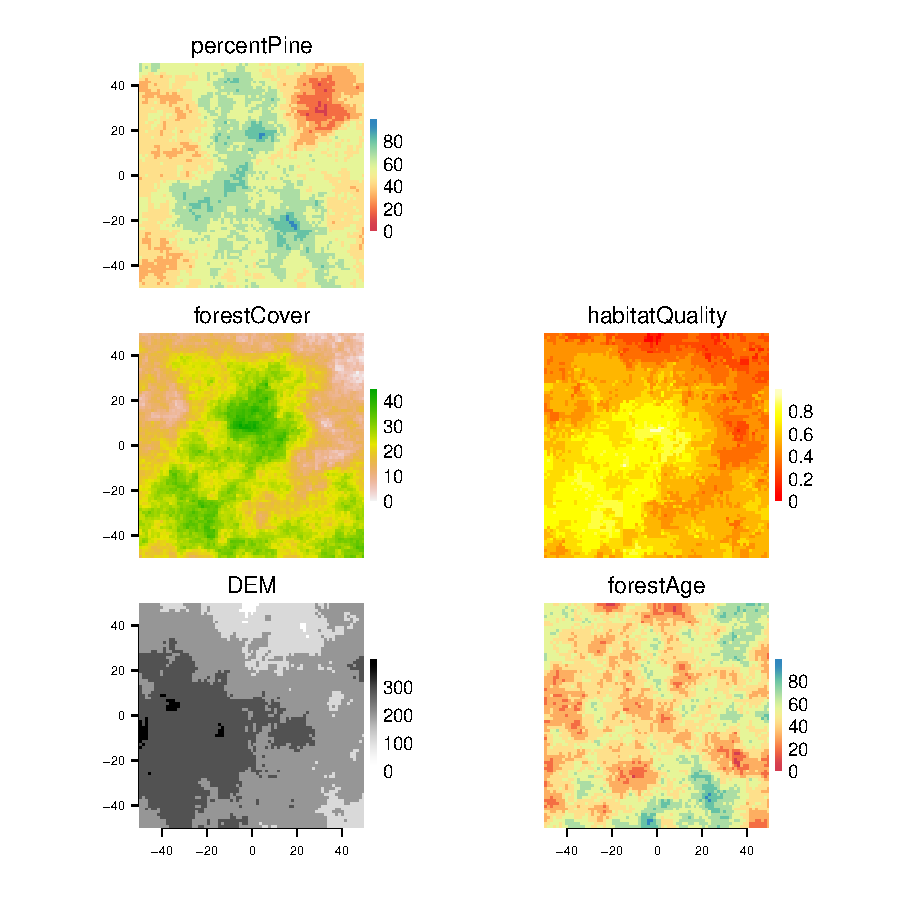
\includegraphics{introduction-habitat-map}

\newpage

\section{Simulating ``agents''}

\paragraph{}
Lorem ipsum ...

\subsection{Spatial agents}

\subsubsection{Point agents}

\paragraph{}
agents represented by a single set of coordinates indicating their current position.

\paragraph{}
Use a \texttt{SpatialPointsDataFrame} with additional columns as needed.

\paragraph{Non-mobile point agents}
e.g., plants

\paragraph{Mobile point agents}
e.g., animals use a \texttt{SpatialPointsDataFrame}, with additonal columns for agents' previous \texttt{n} positions, and any other columns such as age, sex, group membership, etc.

\begin{Schunk}
\begin{Sinput}
> N <- 1e1 # number of agents
> # caribou data vectors
> IDs <- c("Alice", "Bob", "Clark", "Daisy", "Eric",
+          "Franz", "Gabby", "Hayley", "Igor", "Jane")
> sex <- c("female", "male", "male", "female", "male",
+          "male", "female", "female", "male", "female")
> age <- round(rnorm(N, mean=8, sd=3))
> prevX <- runif(N, xmin(habitat)+(ncol(habitat)*0.2), xmax(habitat)-(ncol(habitat)*0.2)) # previous X location
> prevY <- runif(N, ymin(habitat)+(nrow(habitat)*0.2), ymax(habitat)-(nrow(habitat)*0.2)) # previous Y location
> # create the caribou agent object
> caribou <- SpatialPointsDataFrame(coords=cbind(x=rnorm(N, prevX, ncol(habitat)/20),
+                                                y=rnorm(N, prevY, ncol(habitat)/20)),
+                                   data=data.frame(prevX, prevY, sex, age))
> row.names(caribou) <- IDs # alternatively, add IDs as column in data.frame above
> heading(SpatialPoints(cbind(x=prevX,y=prevY)),caribou)
\end{Sinput}
\begin{Soutput}
    Alice       Bob     Clark     Daisy      Eric     Franz     Gabby    Hayley 
 93.46971 292.42703 164.98204 342.89488 273.49100 151.65733 210.22029 303.14473 
     Igor      Jane 
289.69822 139.61266 
\end{Soutput}
\begin{Sinput}
> coordinates(caribou)
\end{Sinput}
\begin{Soutput}
                x          y
Alice   -2.990392   4.264426
Bob     -5.908647  23.523945
Clark   11.254934 -27.433900
Daisy    8.910908   7.488650
Eric   -16.252041  -9.144129
Franz   -6.671158 -28.885787
Gabby  -16.203213  16.954425
Hayley  12.318166  24.271700
Igor   -21.721241  28.202634
Jane    16.614659  -2.508213
\end{Soutput}
\begin{Sinput}
> ## conventional plotting method - agents don't plot properly when it is a raster stack
> #plot(habitat)
> #plot(caribou, add=TRUE)
> 
> # convenient plotting using simPlot
> simPlot(habitat, col=cols[c(2:5,3)])
> simPlot(caribou, on.which.to.plot=c(2,3,5), pch=19, size=unit(0.1,"inches"))
> drawArrows(from=SpatialPoints(cbind(x=prevX, y=prevY)),
+            to=caribou,
+            on.which.to.plot="DEM")
\end{Sinput}
\end{Schunk}
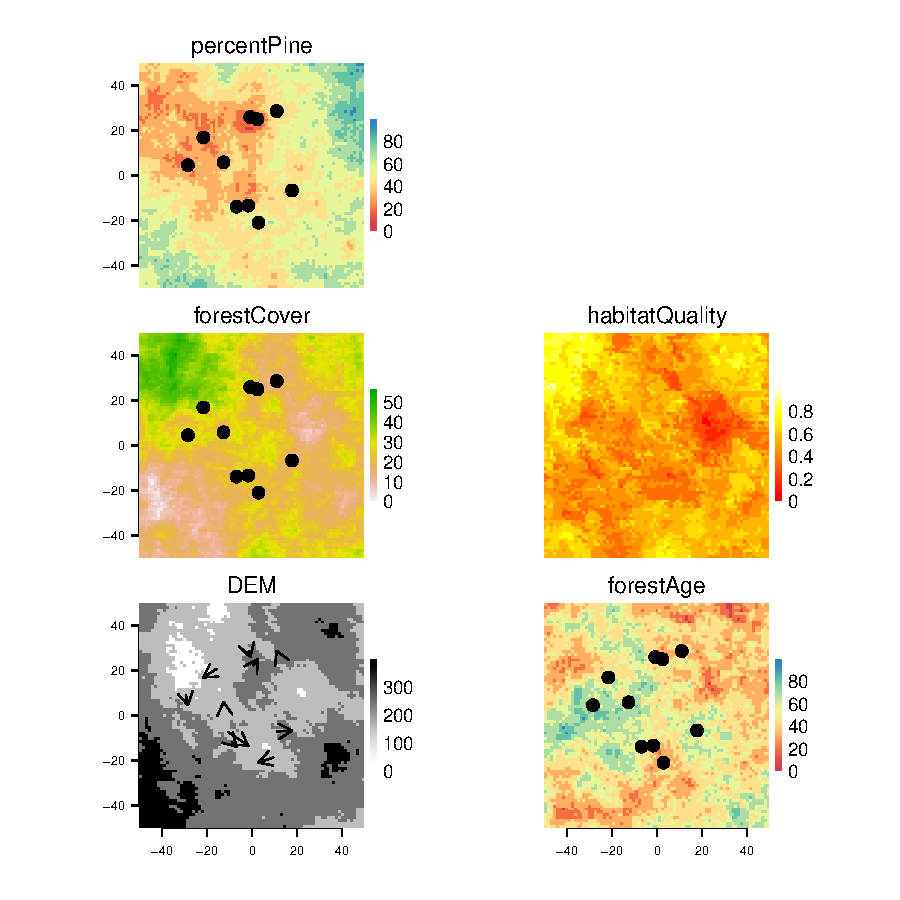
\includegraphics{introduction-mobile-point-agent}

\section{A simple fire model}
\paragraph{Burn some of the forest}
Using the spread function, we can simulate fires, and subsequent changes to the various map layers. Here, spreadProb can be a single probability or a raster map where each pixel has a probability. In the example below, each cell's probability is taken from the Percent Pine map layer.

\begin{Schunk}
\begin{Sinput}
> nFires <- 10 # number of agents
> habitat[["Fires"]] <- spread(habitat[[1]],
+                              loci=as.integer(sample(1:ncell(habitat), nFires)),
+                              spreadProb=0.225,
+                              #spreadProb=habitat[["percentPine"]]/(maxValue(habitat[["percentPine"]])*5)+0.1,
+                              persistance=0,
+                              mapFireID=TRUE,
+                              mask=NULL,
+                              maxSize=1e8,
+                              directions=8,
+                              iterations=1e6,
+                              plot.it=FALSE,
+                              mapID=TRUE)
> simPlot(habitat[["Fires"]])
\end{Sinput}
\end{Schunk}

\paragraph{}


\begin{Schunk}
\begin{Sinput}
> # Show the burning more strongly over abundant pine
> simPlot(habitat[["percentPine"]], col=cols[[3]])
> simPlot(habitat[["Fires"]], add=TRUE, delete.previous=FALSE, col=cols[[1]])
\end{Sinput}
\end{Schunk}
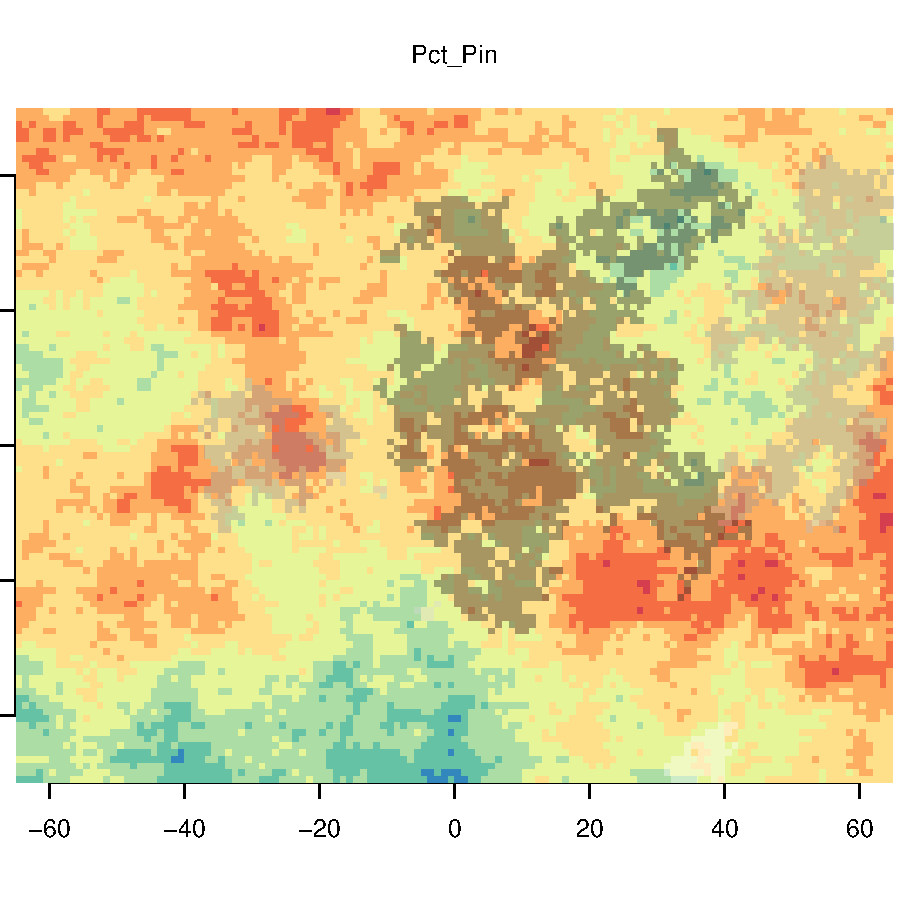
\includegraphics{introduction-fire-overlaid}


\paragraph{}
We can see that the fires tend to be in the Pines because we made it that way, using an arbitrary weighting with pine abundance

\begin{Schunk}
\begin{Sinput}
> # Show the burning more strongly over abundant pine
> fire <- reclassify(habitat[["Fires"]],rcl= cbind(0:1,c(0,ncell(habitat)),0:1))
> pine <- reclassify(habitat[["percentPine"]],rcl= cbind(0:9*10, 1:10*10, 0:9))
> PineByFire <- crosstab(fire, pine, long=TRUE)
> colnames(PineByFire) <- c("fire", "pine", "freq")
> PineByFire$pine <- as.numeric(as.character(PineByFire$pine))
> summary(glm(freq ~ fire*pine, data=PineByFire, family="poisson"))
\end{Sinput}
\begin{Soutput}
Call:
glm(formula = freq ~ fire * pine, family = "poisson", data = PineByFire)

Deviance Residuals: 
    Min       1Q   Median       3Q      Max  
-32.553  -12.885   -2.884   12.256   28.505  

Coefficients:
             Estimate Std. Error z value Pr(>|z|)    
(Intercept)  6.760597   0.020642 327.516   <2e-16 ***
fire1       -2.028387   0.050875 -39.870   <2e-16 ***
pine        -0.033980   0.004047  -8.396   <2e-16 ***
fire1:pine   0.191963   0.008362  22.957   <2e-16 ***
---
Signif. codes:  0 ‘***’ 0.001 ‘**’ 0.01 ‘*’ 0.05 ‘.’ 0.1 ‘ ’ 1

(Dispersion parameter for poisson family taken to be 1)

    Null deviance: 9423.5  on 19  degrees of freedom
Residual deviance: 6364.7  on 16  degrees of freedom
AIC: 6518

Number of Fisher Scoring iterations: 5
\end{Soutput}
\end{Schunk}

\paragraph{}
Sure enough, there are more fires as the abundance of pine goes up, as seen by the positive interaction term (the negative \texttt{fire1} term means that there are more pixels without fires than with fires).

\paragraph{Impact some of the forest}
\begin{Schunk}
\begin{Sinput}
> habitat[["forestAge"]][habitat[["Fires"]]>0] <- 0
> habitat[["forestCover"]][habitat[["Fires"]]>0] <- 0
> habitat[["habitatQuality"]][habitat[["Fires"]]>0] <- 0.1
> habitat[["percentPine"]][habitat[["Fires"]]>0] <- 0
> simPlot(habitat, col=cols[c(2:5,3,1)])
\end{Sinput}
\end{Schunk}
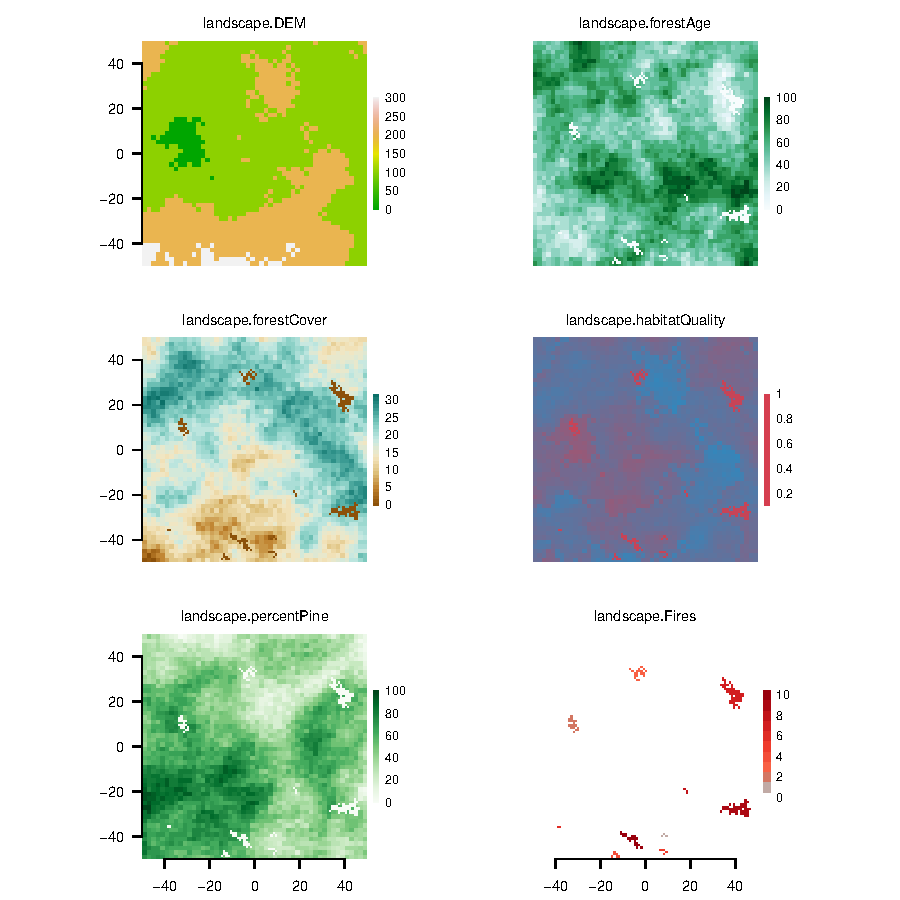
\includegraphics{introduction-fire-impacts-maps}

\section{A simple individual based model (IBM)}
\paragraph{Move some agents}
Using a simple habitat-depedent correlated random walk, simulate the movement of caribou across a heterogeneous landscape. Because we had just had fires, and we assume that fires have a detrimental effect on animal movement, we can see the long steps taken in the new, low quality, post-burn sections of the landscape.

\begin{Schunk}
\begin{Sinput}
> simPlot(habitat[["habitatQuality"]], col=cols[[3]])
> for (i in 1:10) {
+   #crop any caribou that went off maps
+   caribou <<- crop(caribou,habitat)
+   drawArrows(from=SpatialPoints(cbind(x=caribou$prevX, y=caribou$prevY)),
+              to=caribou,length=0.04,
+              on.which.to.plot=1)
+ 
+   # find out what pixels the individuals are on now
+   ex <- habitat[["habitatQuality"]][caribou]
+ 
+   #step length is a function of current cell's habitat quality
+   sl <- 0.25/ex
+ 
+   ln <- rlnorm(length(ex), sl, 0.02) # log normal step length
+   sd <- 30 # could be specified globally in params
+ 
+   caribou <<- crw(caribou, stepLength=ln, stddev=sd, lonlat=FALSE)
+ }
\end{Sinput}
\end{Schunk}
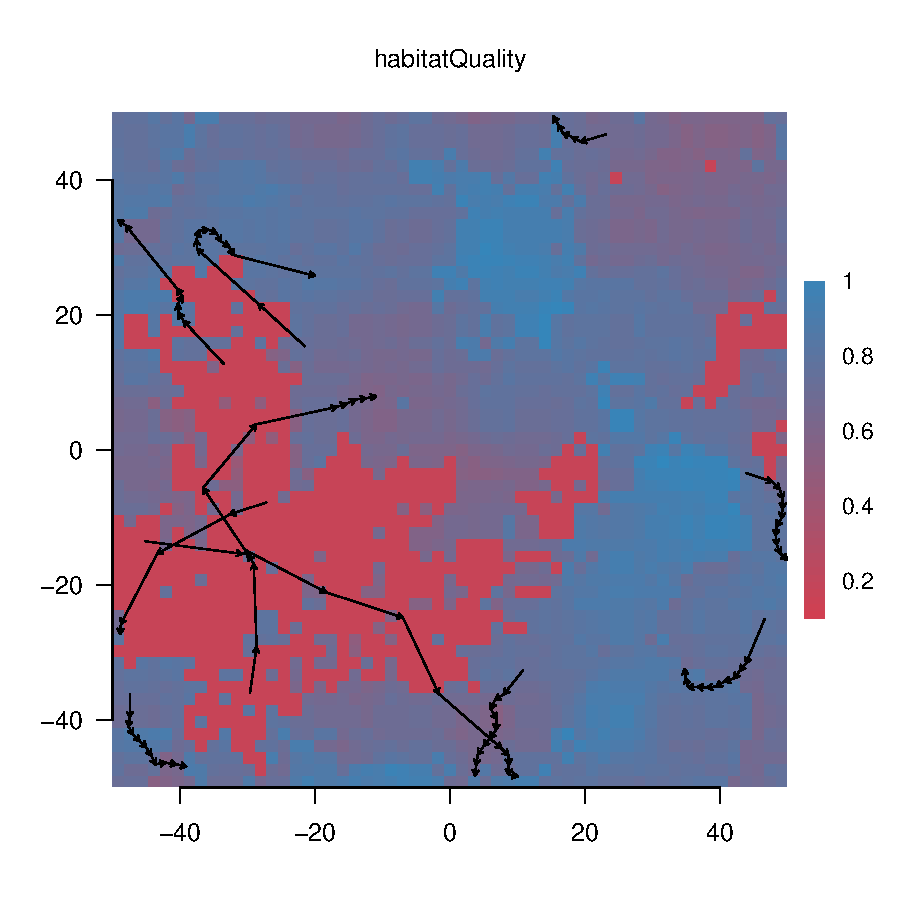
\includegraphics{introduction-agent-crw-trajectory}

\newpage

\section{Further reading}

\subsection{Other \texttt{SpaDES} vignettes:}

%% list all other vignettes here
\begin{itemize}
\item \texttt{modules}: Building modules in \texttt{SpaDES}
\item \texttt{plotting}: Plotting with \texttt{simPlot} in \texttt{SpaDES}
\end{itemize}

\end{document}
